% OUTLINE:
% * Introduction: a bright comet is coming!
% * Observations: COBS, criteria.
% * Light curve analysis: model, model fitting.
% * Discussion & caveats:
%   - compare surface brightness to stars

\documentclass[RNAAS]{aastex63}

%% Define new commands here
\newcommand\latex{La\TeX}
\graphicspath{{./}{figures/}}
\begin{document}

\title{A Probabilistic Brightness Prediction for Comet C/2019 Y4 (ATLAS)}

\correspondingauthor{Geert Barentsen}
\email{hello@geert.io}


\author[0000-0002-3306-3484]{Geert Barentsen}
\affiliation{Bay Area Environmental Research Institute, P.O. Box 25, Moffett Field, CA 94035, USA}

\keywords{Long period comets}


\section{Introduction} \label{sec:intro}

Several media outlets recently reported that comet C/2019 Y4 may soon provide a spectacular \textit{Great Comet} display.
The object was originally discovered on 2019 Dec 28 at magnitude $V\approx19.5$ \citep{CBET4712}. The comet's brightness increased rapidly thereafter, reaching $V\approx8$ by late March (Fig.~\ref{fig:1}). 
The comet is expected to reach peak brightness near its perihelion date on 2020 May 31.
In this research note, we estimate the comet's brightness evolution in a probabilistic way by combining citizen science observations with prior information from previous comets.

\begin{figure}[h!]
\begin{center}
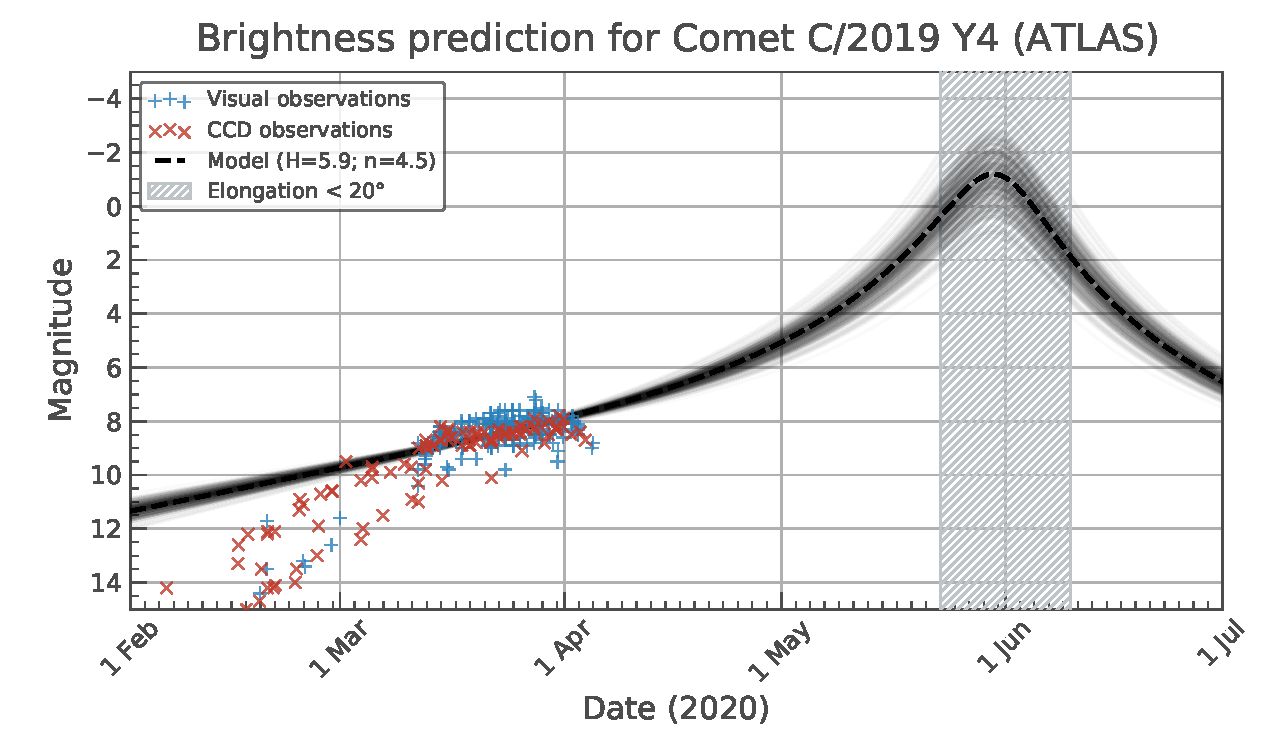
\includegraphics[scale=0.85,angle=0]{2019y4-prediction.pdf}
\caption{Light curve of comet C/2019 Y4. Plusses and crosses show visual and CCD observations from the COBS database. The mean model fit is shown as a thick dashed line. Thin black lines show random MCMC draws to visualize the model uncertainty. The grey hatched area indicates when the comet will be within 20 degrees from the Sun as seen from Earth.\label{fig:1}}
\end{center}
\end{figure}


\section{Observations}

The 
\textit{\href{https://cobs.si}{Comet Observation Database}} \citep[COBS;][]{2018JBAA..128..279Z} contains nearly 250,000 brightness estimates of 1285 comets dating back to 1884. The data are predominantly contributed by citizen scientists.
At the time of writing, the database contained 354 observations of C/2019 Y4 contributed by 52 volunteers across 18 countries.
Fig.~\ref{fig:1} shows the subset of 296 good-quality observations that met the selection criteria\footnote{We use observations reported with the COBS method codes S, B, M, I, E, Z, V, or O. Observations flagged as ``poor'' or ``upper limit'' are excluded.} for our analysis.


\section{Light curve analysis}

The canonical method to model the total magnitude $m$ of a comet (integrated across the coma) as a function of the body's geocentric and heliocentric distances ($\Delta$ and $r$) is a power-law formula in the form
\begin{equation}
m = H + 5 \log{\Delta} + 2.5\,n\,\log{r},
\end{equation}
where $H$ is the absolute magnitude, and $n$ is the \textit{activity index} which is a proxy for the rate of dust production as a function of heliocentric distance. The typical value for $n$ is 4 \citep[][]{2001A&G....42a..11G}, but values exceeding $n>8$ have been reported for segments of light curves associated with enhanced activity \citep[e.g.][]{1990acm..proc..327H}.

We use \texttt{\href{https://docs.pymc.io}{PyMC3}} \citep{pymc} to fit the power law model to the observations in a probabilistic way.
We model the residuals using a zero-centered Cauchy distribution with scale parameter $\beta$.
We adopt empirical Gaussian priors $\beta \sim \mathcal{N}(\mu=0.47,\,\sigma=0.02)\,$, 
$n \sim \mathcal{N}(3.5,\,1.4)\,$,
and
$H \sim \mathcal{N}(6.7,\,2.0)\,$.
We derived these priors by fitting the same model to the 12 brightest long-period comets available in the COBS database.
Finally, we sample the model posterior using the default Markov Chain Monte Carlo algorithm provided by \texttt{PyMC3}.  We verified that changing the priors does not significantly alter the posterior.

\section{Results}

The model light curve corresponding to the mean posterior parameters is shown as a dashed line in Fig.~\ref{fig:1}.
We find a mean value of $n=4.5\pm0.5$ for the activity index, and $H=5.9\pm0.3$ for the absolute magnitude. This corresponds to a peak brightness $m=-1\pm1$ on 2020 May 31. 


\section{Discussion}

Given the current observations and the canonical light curve model, C/2019 Y4 is on track to become the brightest comet since C/2011 W3 (Lovejoy).
We caution the reader for three important caveats however:
\begin{enumerate}
\item The comet will be located very close to the Sun in the sky on 2020 May 31 ($13^o$ elongation). This will severely hinder the comet's visibility.
The observing conditions will be more favorable on or before 2020 May 20 ($24^o$ elongation), but the comet is expected to be much fainter on that date ($m=+1\pm1$).
\item We find that the early observations of the comet prior to mid-March do not fit the canonical model well, suggesting that the activity has decreased over time.
This indicates that the comet's surface may have been covered by a thin layer of volatile materials which have now been depleted. If we exclude the outlier observations recorded prior to 2020 March 15 from the model fit, the expected peak brightness drops significantly to $m=+5\pm1$.
\item Finally, we caution that comets are notoriously difficult to predict.
For example, we cannot exclude the possibility that C/2019 Y4 may break into fragments and brighten dramatically, or conversely, the object may lose its volatiles and fade away more quickly than expected.
\end{enumerate}

%The coma brightness is likely to be spread out across several arcminutes however, likely making the comet look fainter to the eye than a star of a similar brightness.

%In summary, given the current observations and a canonical light curve model, we do not currently expect comet C/2019 Y4 to appear as a \textit{Great Comet}.


The code used in this analysis is available as generic Python package called \texttt{cometcurve} available at \url{github.com/barentsen/cometcurve}. The reader can use this tool to keep track of the comet's evolution.

%The parameter $n$ is able to fit the light curves of many comets in a statistical sense. It is insufficient to capture intricate details in the light curves of comets, which are known to show variability (e.g. cite).


\acknowledgments

The COBS database is the product of the volunteer observers and database maintainers.
The data is available under a Creative Commons Attribution-NonCommercial-ShareAlike 4.0 International License.
% obs = cc.read_cobs(comet="2019Y4", allowed_methods='all')
% ", ".join(obs.observer_name.value_counts().keys())
Specifically, this analysis depends on observations contributed by
Thomas Lehmann, Artyom Novichonok, Denis Buczynski, Steffen Fritsche, Christian Harder, Carl Hergenrother, Piotr Guzik, Maik Meyer, Maciej Kwinta, Nick James, Alex Scholten, Jerzy Bohusz, Johan Warell, David Swan, Mike Collins, Maciej Reszelski, Gerhard Scheerle, Jacek Powichrowski, Martin Masek, Tomasz Sciezor, Gideon van Buitenen, Sandor Szabo, Timo Karhula, Robin Hegenbarth, Nirmal Paul, Marek Biely, Harri Kiiskinen, Piotr Nowak, Andreas Kammerer, Kevin Hills, Volker Kasten, Marcin Filipek, Walter Kutschera, Pavol Dubovsky, Juan Jose Gonzalez Suarez, Jakub Cerny, Pedro Pérez Corujo, Peter De Schrijver, Kristof Friedrich, Teerasak Thaluang, Uwe Pilz, Adam Tuznik, Jose Pablo Navarro Pina, Mikolaj Sabat, Salvador Aguirre, Vladimir Bespalov, Miroslav Lostak, Seiichi Yoshida, Mariusz Swietnicki, Carlos Labordena, Michael Linnolt, and Tibor Csorgei.

\begin{thebibliography}{}

\bibitem[Green et al.(2001)]{2001A&G....42a..11G} Green, D.~W.~E., Marsden, B.~G., \& Morris, C.~S.\ 2001, Astronomy and Geophysics, 42, 1.11

\bibitem[Green(2019)]{CBET4712} Green, D.~W.~E.\ 2019, Central Bureau Electronic Telegrams 4712

\bibitem[Hughes(1990)]{1990acm..proc..327H} Hughes, D.~W.\ 1990, Asteroids, Comets, Meteors III, 327

\bibitem[Salvatier et al.(2016)]{pymc}
Salvatier, J., Wiecki, T.~V., Fonnesbeck, C.\ 2016, PeerJ Computer Science, 2, e55

\bibitem[Tonry et al.(2018)]{2018PASP..130f4505T} Tonry, J.~L., Denneau, L., Heinze, A.~N., et al.\ 2018, \pasp, 130, 064505

\bibitem[Zakrajsek \& Mikuz(2018)]{2018JBAA..128..279Z} Zakrajsek, J., \& Mikuz, H.\ 2018, Journal of the British Astronomical Association, 128, 279

\end{thebibliography}

\end{document}
